DUNE is the flagship of the future US domestic particle physics programme and forms a major part of the UK strategy for participation in the next generation of neutrino oscillation experiments. The 1.2\,MW wide-band neutrino beam, generated by the Long Baseline Neutrino Facility (LBNF) at Fermilab, will be fired 1300\,km towards a 40\,kt fiducial mass liquid argon (LAr) time projection chamber (TPC),  located one mile underground at the Sanford Underground Research Facility (SURF) in South Dakota. 

The deployment of this huge LAr detector, illustrated in Figure~\ref{fig:dune:fardet1}, in an intense neutrino beam will represent a game-changing development in the field of neutrino physics. 

\begin{figure}[!htp]
\centerline{
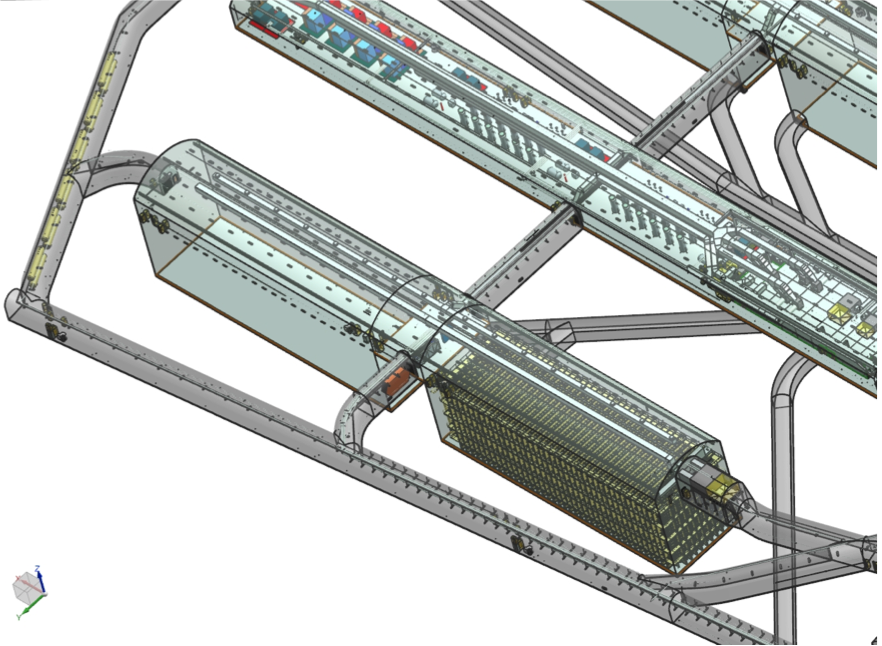
\includegraphics[width=0.7\textwidth]{figs/DUNE_FD.png}
}
\caption[DUNE at SURF]{Illustration of of the underground facility at SURF, showing two of the four underground detector chambers and the central utility cavern. Also shown is the first far detector module (bottom left). To set the scale, the detector chambers are approximately 65\,m long. 
\label{fig:dune:fardet1}}
\end{figure}

In 2014, the US Particle Physics Project Prioritisation Panel (P5) called for the formation of LBNF/DUNE as a truly international project with ambitious scientific goals. LBNF/DUNE was also called out as the highest priority for the US domestic particle physics programme. As a result, the scale and scientific scope of the international LBNF/DUNE project is much greater than that of its predecessor, the US-funded LBNE project. 

LBNF/DUNE was set up as a truly international endeavour from day one -- a first for a US-hosted project of this scale. The international governance model for LBNF and DUNE follows that of the LHC and the LHC experiments. LBNF is the US facility with international contributions at the level of 25\%. DUNE is an international experimental collaboration with an expected US contribution of approximately 25\%. DUNE has broad support from the global particle physics community in the US and Europe and with growing interest in developing countries and Asia. 

LBNF/DUNE passed its DOE CD-1-R review in July 2015, setting the cost for the US contribution at \$1.5B. There is strong support within the US government; both chambers of Congress included authorisation and funding for the LBNF construction start in their FY17 appropriations bills. CD-3a approval for the planned \$300M far site construction was granted in September 2016. This significant milestone marked the approval of the LBNF/DUNE construction, which started in 2017. 

DUNE is strongly supported by CERN who are investing in a large-scale detector prototyping programme at CERN and through a major contribution to the far detector underground facility in South Dakota -- the first time CERN will have invested in an experiment outside CERN. 

While supporting DUNE during the preparatory and pre-construction phases, STFC submitted a business case to BEIS for extra capital and resources to support DUNE, contributions to the facility (LBNF) and the PIP-II accelerator upgrade. The LBNF/DUNE project underwent Gateway Review 0 in the UK, which it passed amber/green. This proposal is putting forward the request for the activities relating to DUNE (WP1-3) as part of the overall LBNF/DUNE project, which also contains the work relating to the target facility (WP4) and the cryo-module for the PIP-II accelerator upgrade (WP5). 